  \pagebreak
  \section{Actividad Práctica}
    Se propone como actividad realizar mediciones de tensión en formas de onda no senoidales,
    empezando por una triangular y una cuadrada, para luego terminar con una proveniente
    de un circuito controlador del ángulo de disparo. Para ello, se hace uso de los siguientes
    insumos:

    \begin{itemize}
      \item Multímetro Escort EDM-82B con detector del valor medio del módulo
      \item Multímetro UT61D con detector True RMS
      \item Generador de funciones GFG-3015
      \item Circuito de control de disparo con triac y diac
      \item Transformador de asilación
      \item Osciloscopio digital Rigol DS1052E
      \item Medidor digital de potencia y factor de potencia
    \end{itemize}
    
    Es importante y obligatorio el uso de un \textbf{transformador de aislación},
    el cual posee una de relación 1:1, y tiene como función crear una barrera física de aislación
    entre los equipos/circuitos con los cuales se trabaja y la red. Esto se justifica con que, la diferencia de
    potencial entre \textit{neutro} y \textit{tierra} de la red no es cero (idealmente debería serlo), para este caso, dicho
    valor es de aproximadamente $\mathbf{1,27\ V}$. Este valor generaría un flujo de corriente a través del osciloscopio 
    directo a la \textit{tierra}, lo cual podría dañar el instrumento, y además, provocaría que el diferencial se active.

      \subsection{Medición de tensión eficaz de ondas no sinusoidales}
    Haciendo uso del generador de funciones se setean señales de forma cuadrada y
    triangular de una amplitud de $5~V_{pp}$ y frecuencia de $50~Hz$. Luego, se 
    mide el valor de tensión con ambos multímetros, se calcula el error, y finalmente,
    se tabula.

    \subsubsection{En una onda cuadrada}
      En la Figura~\ref{fig:SeñalCuadrada} se puede observar la señal cuadrada seteada.
      Luego, en la Figura~\ref{fig:MedicionSeñalCuadrada} se observa la medición de tensión
      con ambos multímetros.

      \begin{figure}[H]
        \centering
        \frame{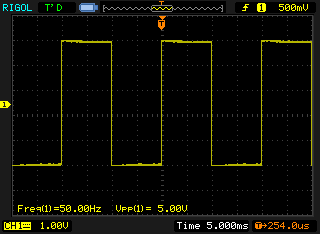
\includegraphics[width=0.48\textwidth]{Imagenes/ActividadPractica/MedicionDeTensionEficaz/Exp1_OndaCuadrada.png}}
        \caption{Señal cuadrada a medir.}
        \label{fig:SeñalCuadrada}
      \end{figure}

      \begin{figure}[H]
        \centering
        \begin{subfigure}[ht]{0.48\textwidth}
          \frame{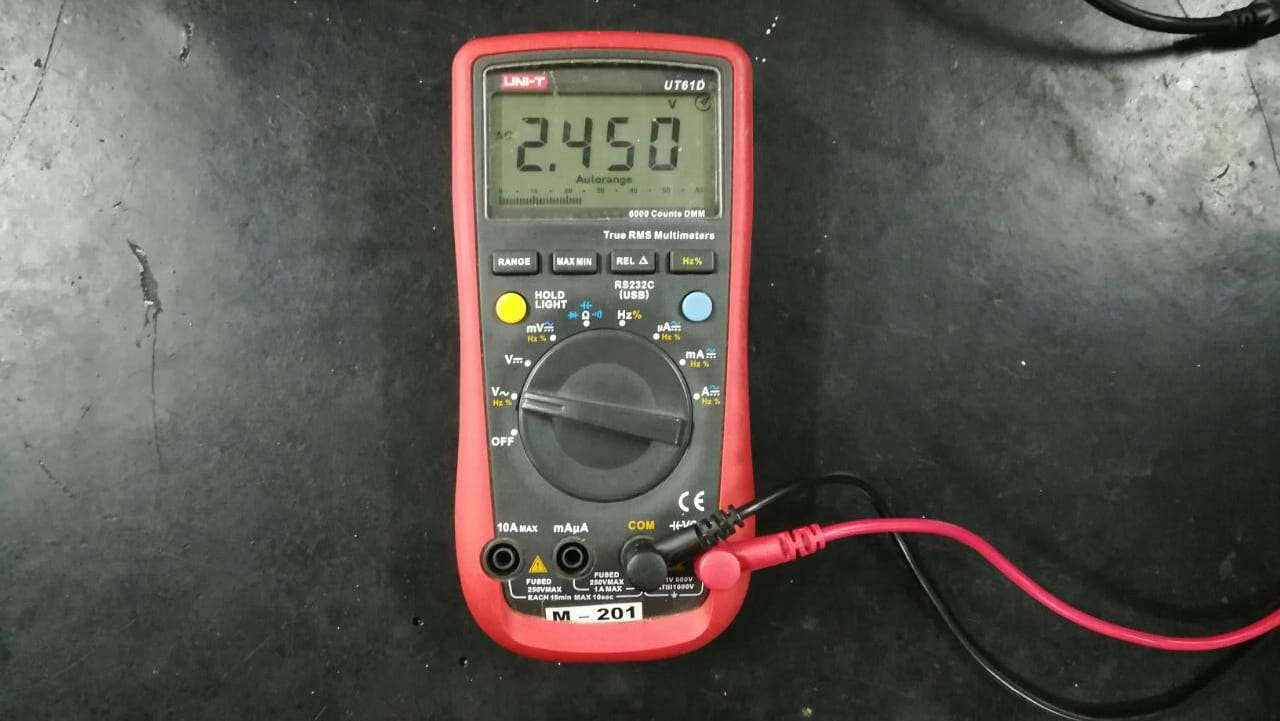
\includegraphics[width=\textwidth]{Imagenes/ActividadPractica/MedicionDeTensionEficaz/Exp1_Vrms_Cuadrada.jpeg}}
          \caption{Medición $V_{RMS}$.}
          \label{fig:MedicionVrmsCuadrada}
        \end{subfigure}
        \hfill 
        \begin{subfigure}[ht]{0.48\textwidth}
          \frame{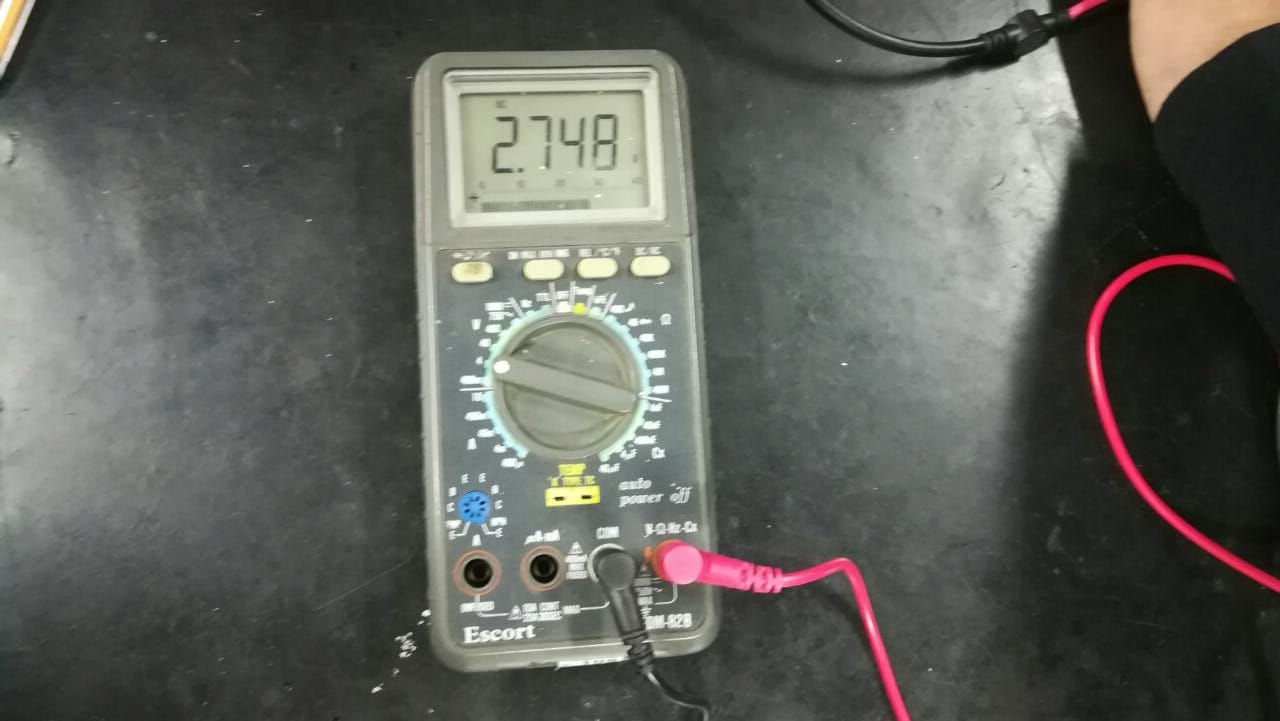
\includegraphics[width=\textwidth]{Imagenes/ActividadPractica/MedicionDeTensionEficaz/Exp1_Vmed_Cuadrada.jpeg}}
          \caption{Medición $V_{|med|}$.}
          \label{fig:MedicionVmedCuadrada}
        \end{subfigure}
        \caption{Mediciones de la señal cuadrada.}
         \label{fig:MedicionSeñalCuadrada}
      \end{figure}


      Luego, la cota de corrección para el multímetro de respuesta al valor medio del módulo es

      \begin{align*}
        e_{cuad} [\%] = \dfrac{V_{RMS} - V_{|med|}}{V_{|med|}} \cdot 100
               = \dfrac{2,450~V - 2,748~V}{2,748V} \cdot 100
               \hspace{20pt} \therefore \hspace{10pt} \Aboxed{e_{cuad} = -10,84\%}~.
      \end{align*}


    \subsubsection{En una onda triangular}
      En la Figura~\ref{fig:SeñalTriangular} se puede observar la señal triangular seteada.
      Luego, en la Figura~\ref{fig:MedicionSeñalTriangular} se observa la medición de tensión
      con ambos multímetros.

      \begin{figure}[H]
        \centering
        \frame{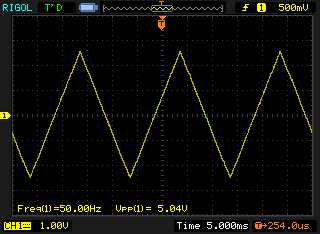
\includegraphics[width=0.45\textwidth]{Imagenes/ActividadPractica/MedicionDeTensionEficaz/Exp1_OndaTriangular.png}}
        \caption{Señal triangular a medir.}
        \label{fig:SeñalTriangular}
      \end{figure}

      \begin{figure}[H]
        \centering
        \begin{subfigure}[ht]{0.48\textwidth}
          \frame{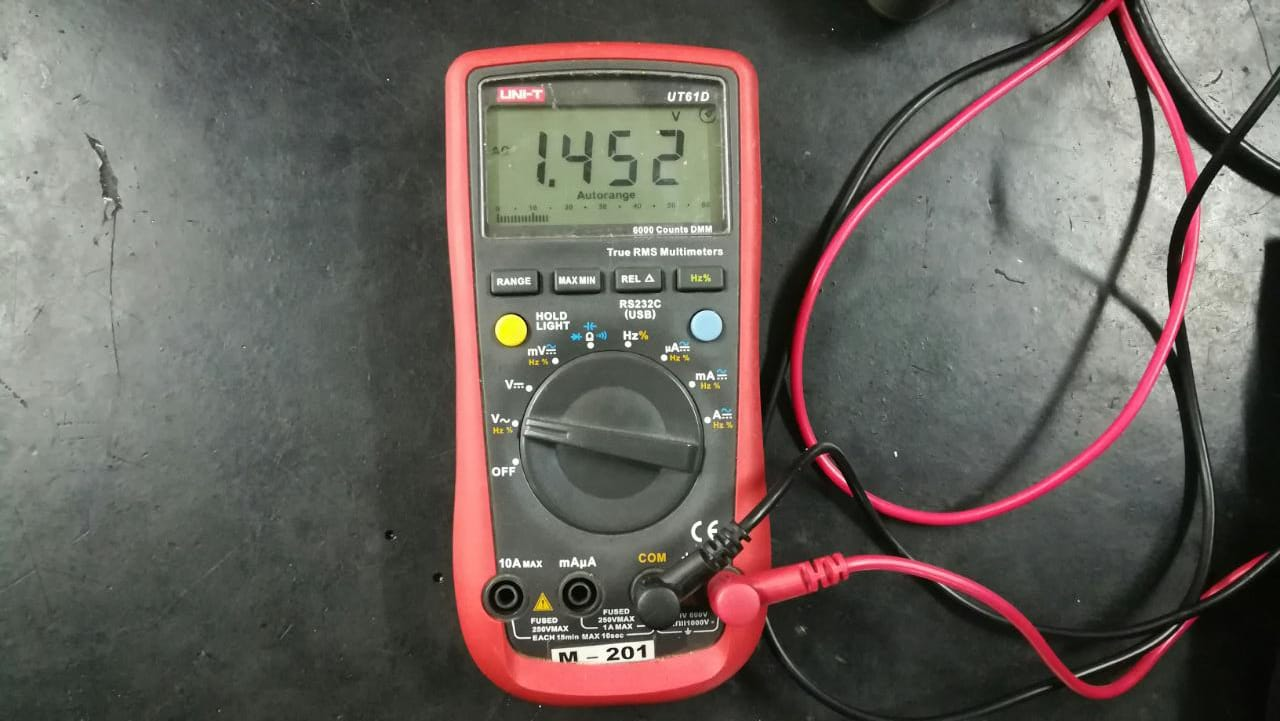
\includegraphics[width=\textwidth]{Imagenes/ActividadPractica/MedicionDeTensionEficaz/Exp1_Vrms_Triangular.jpeg}}
          \caption{Medición $V_{RMS}$.}
          \label{fig:MedicionVrmsTriangular}
        \end{subfigure}
        \hfill 
        \begin{subfigure}[ht]{0.48\textwidth}
          \frame{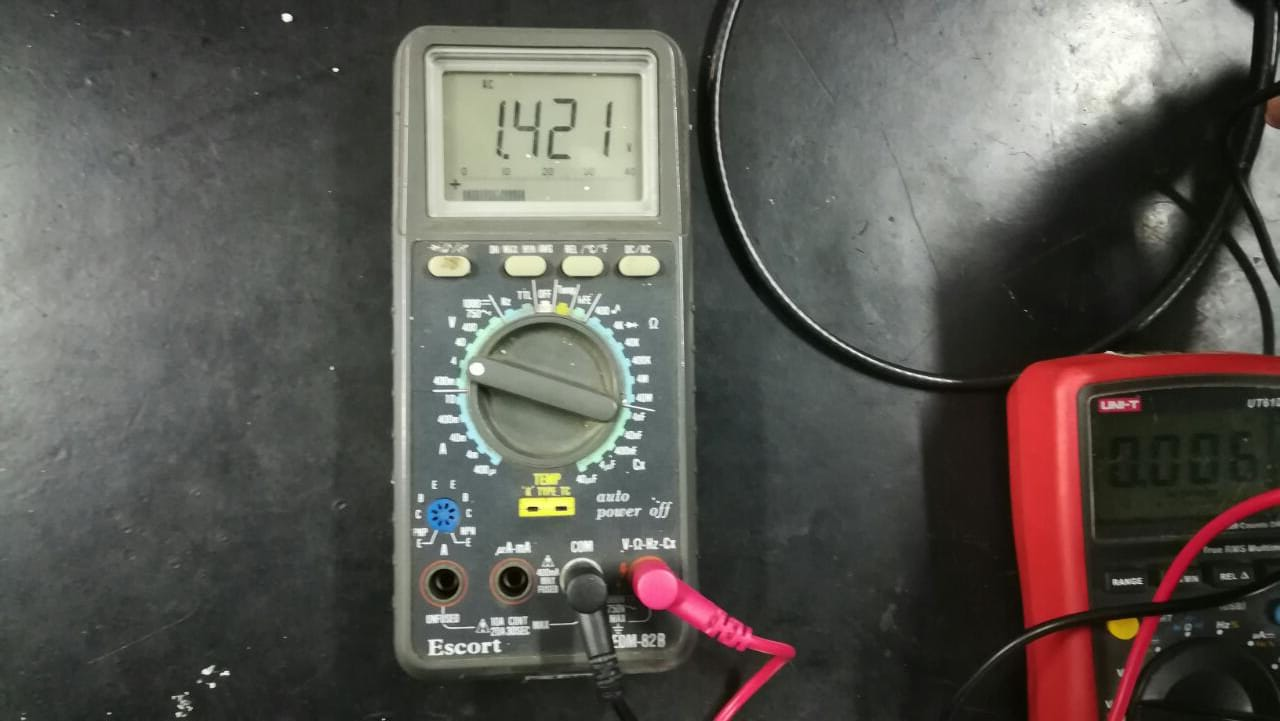
\includegraphics[width=\textwidth]{Imagenes/ActividadPractica/MedicionDeTensionEficaz/Exp1_Vmed_Triangular.jpeg}}
          \caption{Medición $V_{|med|}$.}
          \label{fig:MedicionVmedTriangular}
        \end{subfigure}
        \caption{Mediciones de la señal triangular.}
         \label{fig:MedicionSeñalTriangular}
      \end{figure}

      Luego, la cota de corrección para el multímetro de respuesta al 
      valor medio del módulo es

      \begin{align*}
        e_{tri} [\%] = \dfrac{V_{RMS} - V_{|med|}}{V_{|med|}} \cdot 100
               = \dfrac{1,452~V - 1,421~V}{1,421~V} \cdot 100
               \hspace{20pt} \therefore \hspace{20pt} \Aboxed{e_{tri}= +2,18\%}~.
      \end{align*}

    Los resultados de este experimento se encuentran consignados en la
    Tabla~\ref{tab:MedicionesOndasCuadYTrian}.
  
    \begin{table}[H] \centering
      \begin{tabular}{|c|c|c|c|} \hline
        \textbf{Señal}     & \textbf{Lectura RMS [V]}  & \textbf{Lectura |med| [V]} & \textbf{e [\%]} \\ \hline
      $\mathbf{Cuadrada~(50~Hz - 5~V_{pp})}$    & 2,450     & 2,748         &  -10,84        \\ \hline
      $\mathbf{Triangular~(50~Hz - 5~V_{pp})}$  & 1,452      & 1,421        &  +2,18         \\ \hline
      \end{tabular}
      \caption{Tabla de mediciones y cotas de corrección.}
      \label{tab:MedicionesOndasCuadYTrian}
    \end{table}

      \subsection{Medición de la tensión eficaz de una onda proveniente de un circuito de control de ángulo de conducción}
Para la siguiente parte del experimento, se utiliza un circuito de medición 
de ángulo de disparo. El mismo se enseña en la Figura \ref{fig:CircuitoTriac}.

\begin{figure}[H]
  \centering
  \frame{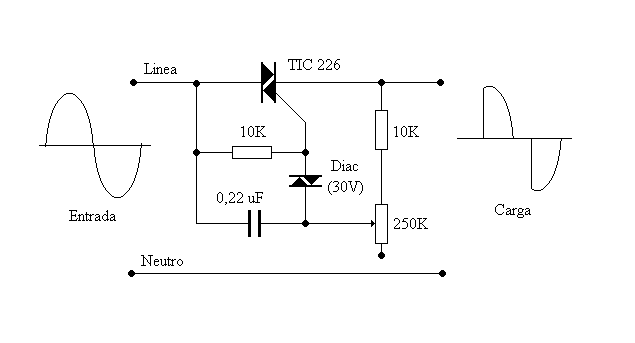
\includegraphics[width=0.6\textwidth]{Imagenes/ActividadPractica/MedicionDeTensionEficazConCircuitoTriac/Esquema_Circuito_Angulo_Disparo.png}}
  \caption{Esquema del circuito de control de ángulo de disparo.}
  \label{fig:CircuitoTriac}
\end{figure}

El procedimiento consiste en medir la tensión de entrada al circuito, 
y medir la de salida sobre la carga, tomando lecturas
al variar el ángulo de conducción con un multímetro que mide True RMS y otro de valor medio. 
Luego se debe confeccionar un gráfico normalizado de tension de salida 
respecto de la entrada, con las curvas obtenidas con cada instrumento.

El esquema de conexión se presenta a continuación en la Figura \ref{fig:EsquemaConexionTriac}.

\begin{figure}[H]
  \centering
  \frame{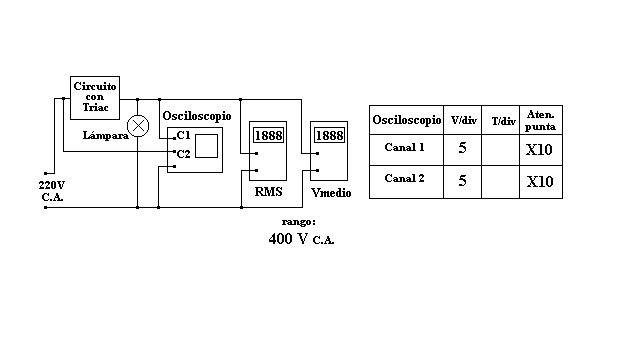
\includegraphics[width=0.5\textwidth]{Imagenes/ActividadPractica/MedicionDeTensionEficazConCircuitoTriac/Esquema_Conexion_Circuito_Angulo_Disparo.png}}
  \caption{Esquema de conexión para el relevamiento de curva.}
  \label{fig:EsquemaConexionTriac}
\end{figure}

Se presentan a continuación los valores tabulados.

\begin{table}[H]
\centering
  \begin{tabular}{|c|c|c|c|c|}
    \hline
      Fase & $Vo_1$[V] & $Vo_2$[V] & $(\frac{Vo_1}{V_{in}})$[V] & $(\frac{Vo_2}{V_{in}})$[V] \\
    \hline
      0°    & 234     & 234     & 1,064   & 1,064\\
      36°   & 222,8   & 211,6   & 1,013   & 0,962\\
      72°   & 194,5   & 158,6   & 0,884   & 0,721\\
      108°  & 135,8   & 189,6   & 0,617   & 0,407\\
      144°  & 58,77   & 30,0    & 0,267   & 0,136\\
      180°  & 0       & 0       & 0       & 0\\
    \hline
  \end{tabular}
\end{table}

Finalmente, se confecciona un gráfico con los valores obtenidos, 
donde se visualizan las curvas de los instrumentos.

\begin{figure}[H]
  \centering
  \frame{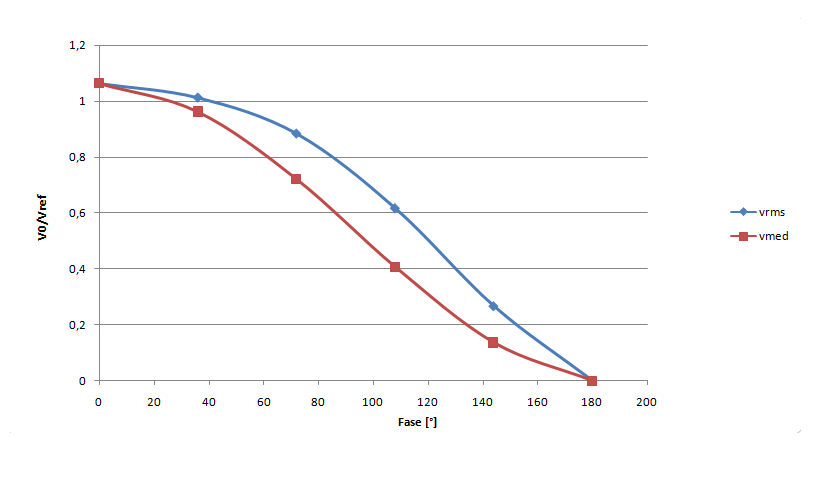
\includegraphics[width=1\textwidth]{Imagenes/ActividadPractica/MedicionDeTensionEficazConCircuitoTriac/Grafico_Contrastacion.png}}
  \caption{Gráfico obtenido.}
  \label{fig:CurvaTrueMedio}
\end{figure}




      \subsection{Medición de factor de potencia en un circuito con control de ángulo de conducción}

Para el siguiente experimento se emplea el mismo circuito de la sección anterior. 
Ésta vez se conecta al medidor digital para medir 
el factor de potencia.

\begin{figure}[H]
  \centering
  \frame{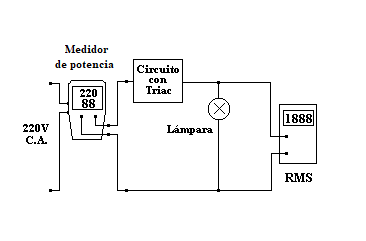
\includegraphics[width=0.5 \textwidth]{Imagenes/ActividadPractica/MedicionDeFactorDePotenciaConCircuitoTriac/Circuito_Medicion_FP_TriacDiac.png}}
  \caption{Circuito de medición de factor de potencia.}
  \label{fig:CircuitoMideFDP}
\end{figure}

Una vez realizada la conexión, se debe variar el potenciómetro del circuito 
de control de disparo, hasta lograr que la tensión eficaz de 
salida sea de 110~V.

\begin{figure}[H]
  \centering
  \frame{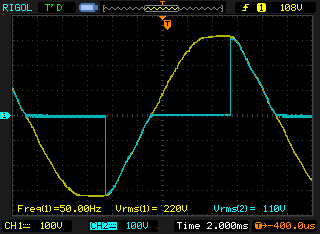
\includegraphics[width=0.5 \textwidth]{Imagenes/ActividadPractica/MedicionDeFactorDePotenciaConCircuitoTriac/Exp3_AnguloDisparoPara110Vrms.png}}
  \caption{Forma de onda para una tensión eficaz de 110[V].}
  \label{fig:SeñalExp3}
\end{figure}

 En éste punto se mide el factor de potencia inicial, 
 cuyo valor es de 0,47.

 \begin{figure}[H]
  \centering
  \frame{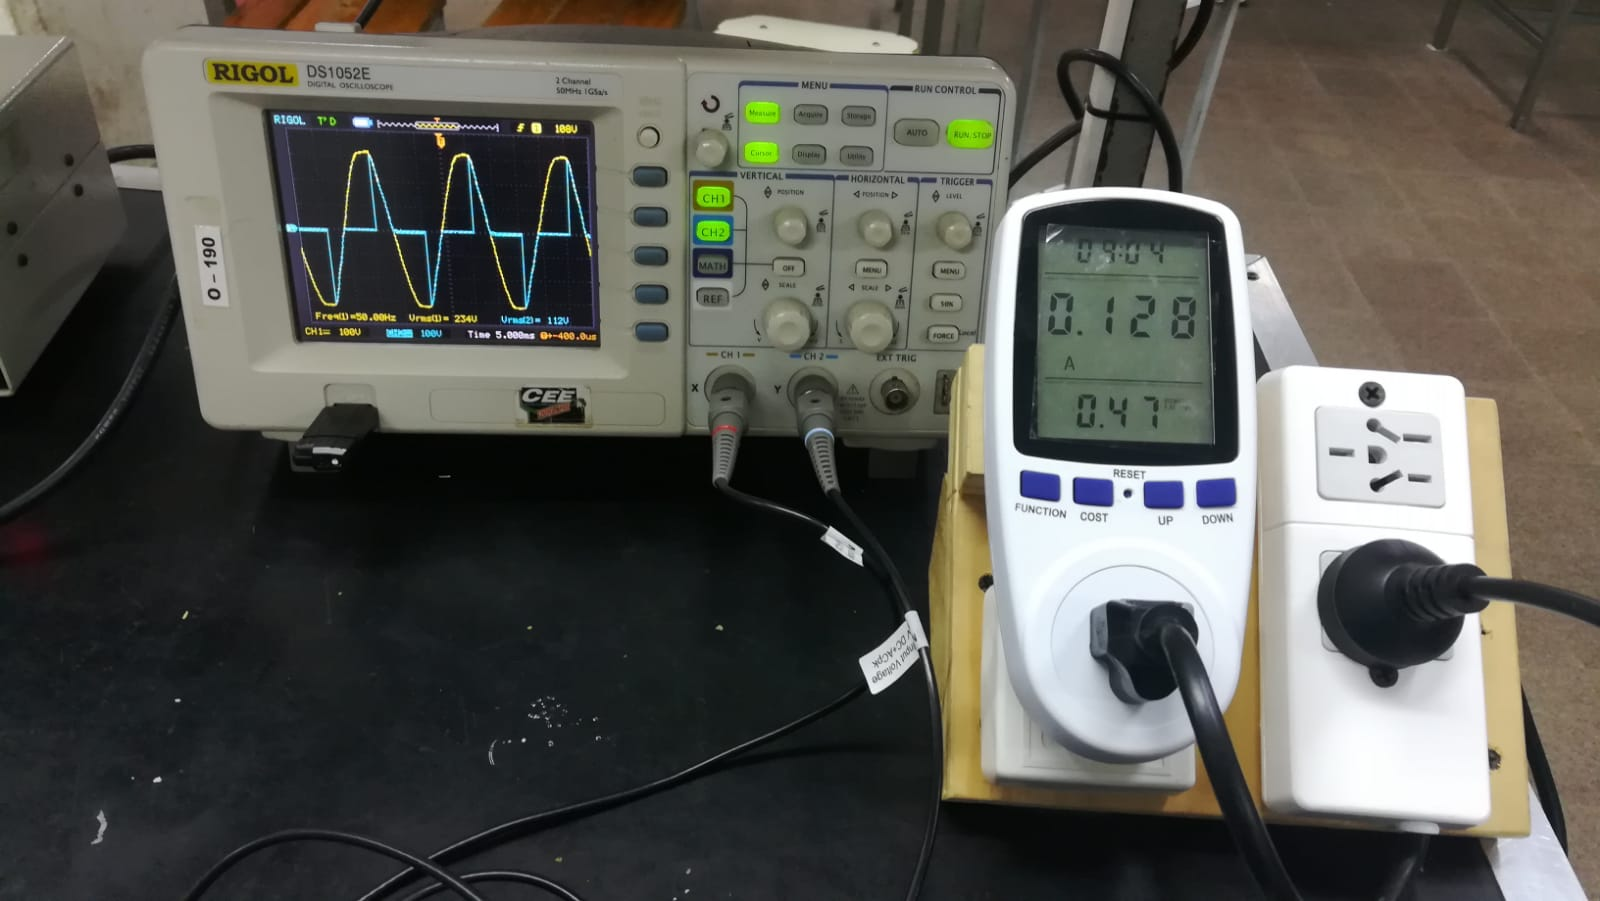
\includegraphics[width=0.5 \textwidth]{Imagenes/ActividadPractica/MedicionDeFactorDePotenciaConCircuitoTriac/Exp3_FDPcon110Vrms.jpeg}}
  \caption{Factor de potencia inicial.}
  \label{fig:FDPExp3}
\end{figure}

Al conectar el capacitor de corrección, se observa que el factor 
de potencia aumenta a 0,55, como muestra la Figura~\ref{fig:FDPCorregidoExp3}. 
Ésto indica que la carga total del circuito en conjunto, se comporta de manera inductiva.

 \begin{figure}[H]
  \centering
  \frame{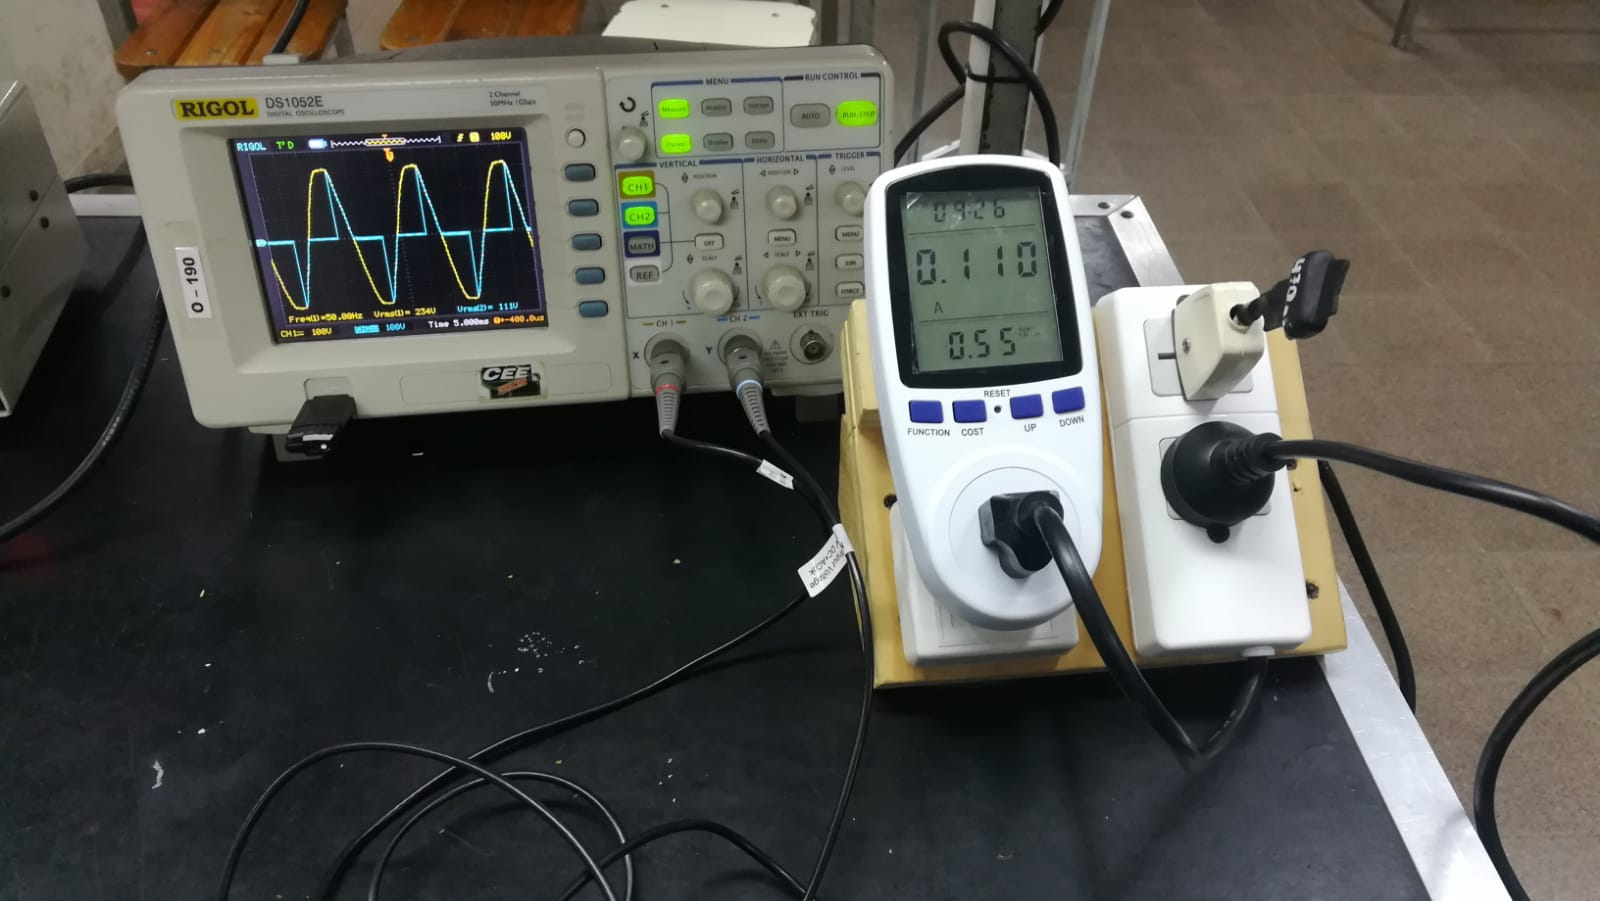
\includegraphics[width=0.5 \textwidth]{Imagenes/ActividadPractica/MedicionDeFactorDePotenciaConCircuitoTriac/Exp3_FDPConCapacitor.jpeg}}
  \caption{Factor de potencia corregido.}
  \label{fig:FDPCorregidoExp3}
\end{figure}

